\begin{figure}[ht]
\tikzset{white/.style={shape=circle,draw=black,fill=white,inner sep=1pt, minimum size=7pt}}
\tikzset{starnode/.style={inner sep=1pt, minimum size=7pt, star,star points=4,star point ratio=0.5, draw, fill=white}}
\tikzset{invisible/.style={shape=circle,draw=black,fill=black,inner sep=0pt, minimum size=0.1pt}}


\begin{center}
\hskip 6mm

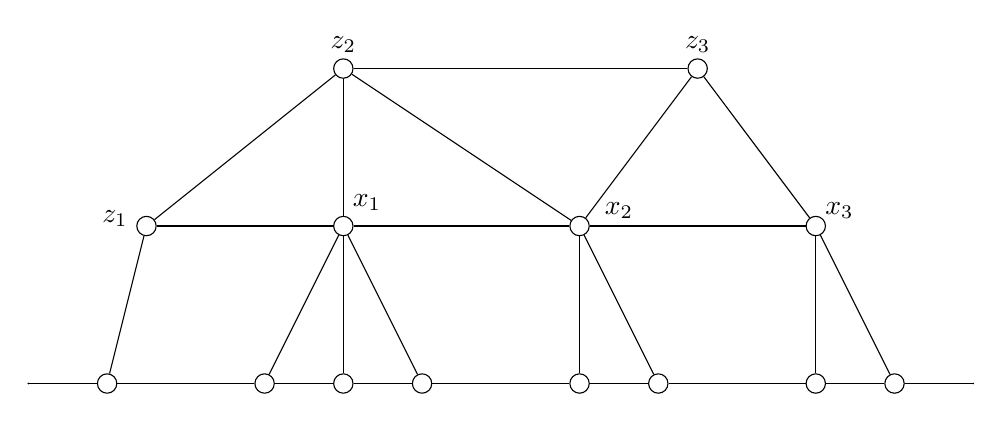
\begin{tikzpicture}
        \node[white] (1) at (1,0){};
        \node[white] (2) at (3,0){};
        \node[white] (3) at (4,0){};
        \node[white] (4) at (5,0){};
        \node[white] (5) at (7,0){};
        \node[white] (6) at (8,0){};
        \node[white] (7) at (10,0){};
        \node[white] (8) at (11,0){};
        \node[white] (9) at (1.5,2){};
        \node[] at (1.1,2.1){$z_1$};
        \node[white] (10) at (4,2){};
        \node[] at (4.3,2.3){$x_1$};
        \node[white] (11) at (7,2){};
        \node[] at (7.5,2.2){$x_2$};
        \node[white] (12) at (10,2){};
        \node[] at (10.3,2.2){$x_3$};
        \node[white] (13) at (4,4){};
        \node[] at (4,4.3){$z_2$};
        \node[white] (14) at (8.5,4){};
        \node[] at (8.5,4.3){$z_3$};
       \node[invisible] (15) at (0,0){};
        \node[invisible] (16) at (12,0){};

        \draw[black] (1)--(2);
        \draw[black] (2)--(3);
        \draw[black] (3)--(4);   
        \draw[black] (4)--(5); 
        \draw[black] (5)--(6); 
        \draw[black] (6)--(7); 
        \draw[black] (7)--(8); 
        \draw[black] (9)--(10);
        \draw[black] (10)--(11);
        \draw[black] (11)--(12);
        \draw[black] (13)--(14);

        \draw[black] (1)--(9);
        \draw[black] (2)--(10);
        \draw[black] (3)--(10);
        \draw[black] (4)--(10);
        \draw[black] (5)--(11);
        \draw[black] (6)--(11);
        \draw[black] (7)--(12);
        \draw[black] (8)--(12);

        \draw[black] (9)--(13);
        \draw[black] (10)--(13);
        \draw[black] (11)--(13);
        \draw[black] (11)--(14);
        \draw[black] (12)--(14);
        \draw[black] (15)--(1);  
        \draw[black] (16)--(8);  
        
\end{tikzpicture}
\caption{Vertices $z_1$, $z_2$, and $z_3$ as described in Claims \ref{x2nbrpath} and \ref{degx3}. For each $i \in \{1,2,3\}$, the vertex $x_i$ is in $X_i$. Moreover, $x_2$ is of type (1,0,0), and $x_3$ is of type (2,0,0).}
    \label{fig:z1z2z3}
\end{center}
\end{figure}






